\documentclass[usenames,dvipsnames]{beamer}
\usepackage{xcolor,booktabs}
\usepackage{listings}
\usetheme{Madrid}
\beamertemplatenavigationsymbolsempty
\begin{document}
\author{Md.Al-Helal, 2018-19}
\institute[CSEDU]{Computer Science \& Engineering\\University of Dhaka}
\title{Chapter 10 : Tracking and Motion}
\date{May 16, 2018}
\begin{frame}
  \maketitle
\end{frame}
\begin{frame}
\frametitle{The Basics of Tracking}
Understanding the motion of a object has two main components:
\begin{itemize}
\item \textbf{Identification}\\
Finding the object of interest from one frame in a subsequent
frame of the video stream.
\begin{itemize}
\item Momemnts
\item Coloer Histogram
\end{itemize}
Tracking unidentified objects is important when we wish to determine what is interesting based on its motion.
\begin{itemize}
\item Lucas-Kanade
\item Horn-Schunck
\end{itemize}
\item \textbf{Modeling}\\
Provides a noisy measurement of the object’s actual position.Many
powerful mathematical techniques have been developed for this. These methods are applicable to 2D or 3D objects and their locations.
\end{itemize}
\end{frame}
\begin{frame}[allowframebreaks]
\frametitle{Corner Finding}
\begin{itemize}
\item If we pick a \textbf{point on a large blank wall} then it won’t be easy to find that same point in the next frame of a video.
\item If all points on the wall are \textbf{identical or even very similar}, then we won’t have much luck tracking that point in subsequent frames.
\item On the other hand, if we choose a point that is \textbf{unique} then we have a pretty \textbf{good chance} of finding that point again.\\

In practice, the point or feature we select should be \textbf{unique, or nearly unique}, and should be \textbf{parameterizable} in such a way that it can be \textbf{compared} to other points in another image.
\end{itemize}
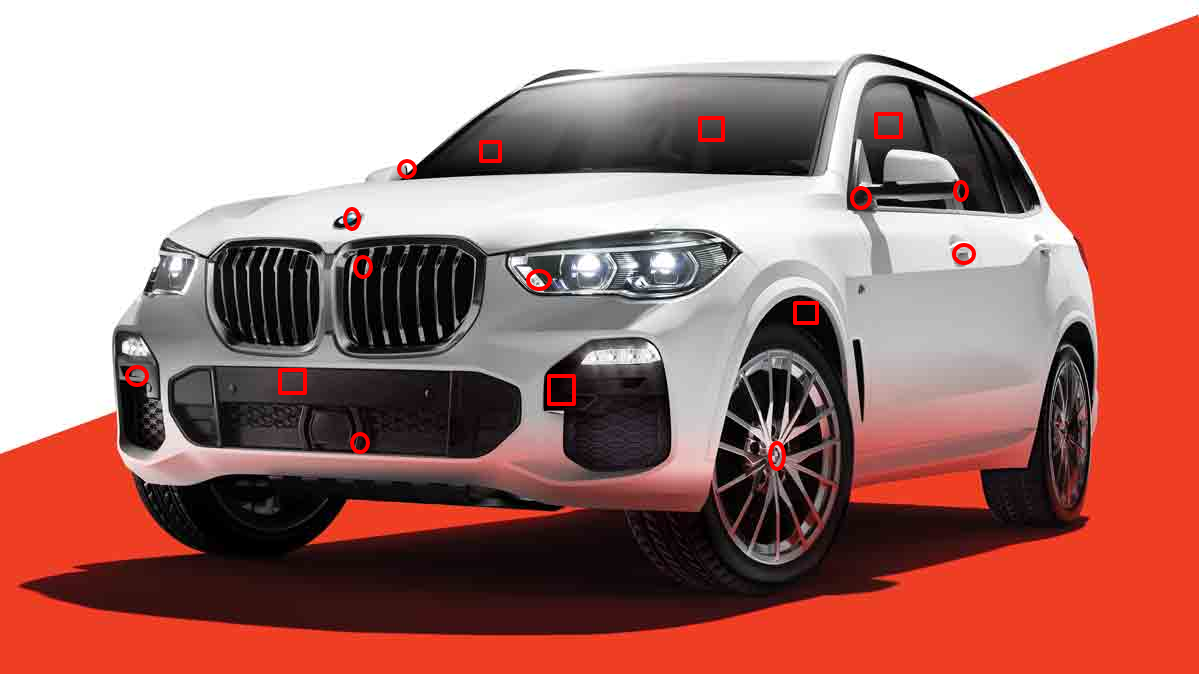
\includegraphics[scale=.30]{Images/car.png}

\framebreak
\textbf{How we can find the corners?}\\
If strong derivatives are observed in two orthogonal directions then we can hope that this point is more likely to be unique. For this reason, many trackable features are called \textbf{corners} ( corners are not edges ).

The cvGoodFeaturesToTrack() function computes the second derivatives (using the Sobel operators) and returns a list of the
points that meet our definition of being good for tracking.
\end{frame}
\begin{frame}[fragile]
\frametitle{Code}
\begin{lstlisting}[language=c]
void cvGoodFeaturesToTrack(
	const CvArr*  	image,
	CvArr*        	eigImage,
	CvArr*          tempImage,
	CvPoint2D32f*   corners,
	innt*           corner_count,
	double          quality_level,
	double          min_distance,
	const CvArr*    mask = NULL,
	int             block_size   = 3,
	int             use_harris   = 0,
	double          k            = 0.4
);
\end{lstlisting}
\vspace{-0.9cm}
\begin{table}
\footnotesize
\begin{tabular}{ll}
tempImage and eigImage & Used as scratch by the algorithm\\
corners & contain the result points after the algorithm has run\\
corner\_count & indicates the maximum number of points\\
quality\_level & indicates the minimal acceptable lower eigenvalue for a point to be included as a corner\\
min\_distance & guarantees that no two returned points are within the indicated number of pixels.
\end{tabular}
\end{table}
\end{frame}
\begin{frame}[allowframebreaks]
\frametitle{Optical Flow}
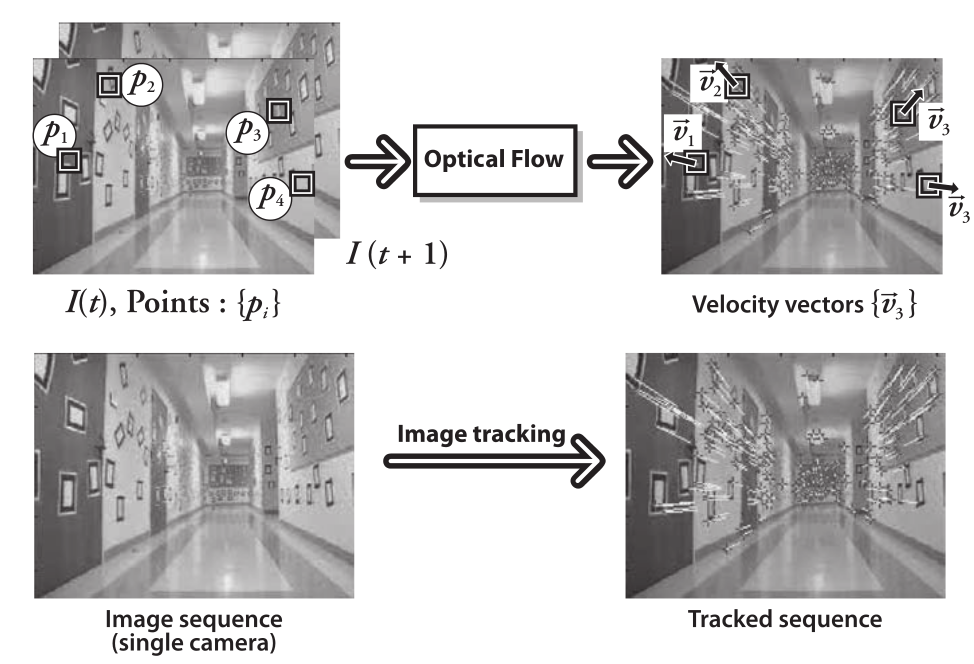
\includegraphics[scale=.32]{Images/pic_hall.png}
\begin{itemize}
\item \textbf{Dense optical flow}\\
Find velocity or displacement for all pixel between previous and current frame. Horn-Schunck method and the block matching method.
\item \textbf{Sparse optical flow}\\
Find velocity or displacement for subset of pixel those have certain desirable properties such as 'corners'. Most popular sparse tracking technique, Lucas-Kanade (LK) optical flow.
\end{itemize}
\end{frame}

\begin{frame}[fragile]
\frametitle{Optical Flow (Dense Optical Flow)}
\framesubtitle{Horn-Schunck technique code}
\begin{lstlisting}[language=c]
void cvCalcOpticalFlowHS(
	const CvArr*      imgA,
	const CvArr*      imgB,
	int               usePrevious,
	CvArr*            velx,
	CvArr*            vely,
	double            lambda,
	CvTermCriteria    criteria
);
\end{lstlisting}
\begin{tabular}{ll}
lambda & Lagrange multiplier\\
usePrevious & tells the algorithm to use the velx and vely velocities
computed from a previous frame as the initial starting point for computing the new velocities\\
criteria & termination criteria\\
\end{tabular}
\end{frame}
\begin{frame}[fragile]
\frametitle{Optical Flow ( Dense Optical Flow )}
\framesubtitle{Block matching code}
\begin{lstlisting}[language=c]
void cvCalcOpticalFlowBM(
	const CvArr*       prev,
	const CvArr*       curr,
	CvSize             block_size,
	CvSize             shift_size,
	CvSize             max_range,
	int                use_previous,
	CvArr*             velx,
	CvArr*             vely
);
\end{lstlisting}
\begin{tabular}{ll}
block\_size & size of the block to be used\\
shift\_size & step size between blocks\\
max\_range & size of the region around a given block that will be searched for a corresponding block in the subsequent frame\\
\end{tabular}
\end{frame}
\begin{frame}[fragile]
\frametitle{Optical Flow (Sparse Optical flow)}
\framesubtitle{Lucas-Kanade code}
\begin{lstlisting}[language=c]
void cvCalcOpticalFlowLK(
	const CvArr*    imgA,
	const CvArr*    imgB,
	CvSize          winSize,
	CvArr*          velx,
	CvArr*          vely
);
\end{lstlisting}
\begin{tabular}{ll}
winSize & window used for
computing the local coherent motion\\
\end{tabular}
\end{frame}
\begin{frame}{\phantom{}}
 % \color{Brown}
  \color{Sepia}
  \centering \Huge\textbf{Thank You}
\end{frame}

\end{document}
